\documentclass[11pt,letterpaper]{article}

\addtolength{\oddsidemargin}{-.875in}
\addtolength{\evensidemargin}{-.875in}
\addtolength{\textwidth}{1.75in}

\addtolength{\topmargin}{-.875in}
\addtolength{\textheight}{1.75in}

\usepackage[utf8]{inputenc}
\usepackage{caption} % for table captions
\usepackage{amsmath} % for multi-line equations and piecewises
\DeclareMathOperator{\sign}{sign}
\usepackage{graphicx}
\usepackage{relsize}
\usepackage{xspace}
\usepackage{verbatim} % for block comments
\usepackage{subcaption} % for subfigures
\usepackage{enumitem} % for a) b) c) lists
\newcommand{\Cyclus}{\textsc{Cyclus}\xspace}%
\newcommand{\Cycamore}{\textsc{Cycamore}\xspace}%
\newcommand{\deploy}{\texttt{d3ploy}\xspace}%
\newcommand{\Deploy}{\texttt{D3ploy}\xspace}%
\usepackage{tabularx}
\usepackage{color}
\usepackage{multirow}
\usepackage{float} 
\usepackage[acronym,toc]{glossaries}
%\include{acros}
\definecolor{bg}{rgb}{0.95,0.95,0.95}
\newcolumntype{b}{X}
\newcolumntype{f}{>{\hsize=.15\hsize}X}
\newcolumntype{s}{>{\hsize=.5\hsize}X}
\newcolumntype{m}{>{\hsize=.75\hsize}X}
\newcolumntype{r}{>{\hsize=1.1\hsize}X}
\usepackage{titling}
\usepackage[hang,flushmargin]{footmisc}
\renewcommand*\footnoterule{}
\usepackage{tikz}

\usetikzlibrary{shapes.geometric,arrows}
\tikzstyle{process} = [rectangle, rounded corners, 
minimum width=1cm, minimum height=1cm,text centered, draw=black, 
fill=blue!30]
\tikzstyle{arrow} = [thick,->,>=stealth]

\graphicspath{}

\begin{document}

\section{Pseudo-1D-neutronics}

The geometries are 2D stripes.
The BCs in the x-direction is homogeneous Neumann on both sides.
Thus, it is like if we were solving for the 1D case.

\subsection{2D-fuel-action}

	\begin{itemize}
		\item Input file: \textit{2D-fuel-action.i}
		\item Mesh: \textit{2D-fuel.msh}
		\item Transient problem.
	\end{itemize}

Figure \ref{fig:2D-fuel-action} shows the results.

	\begin{figure}[htbp!]
		\centering
		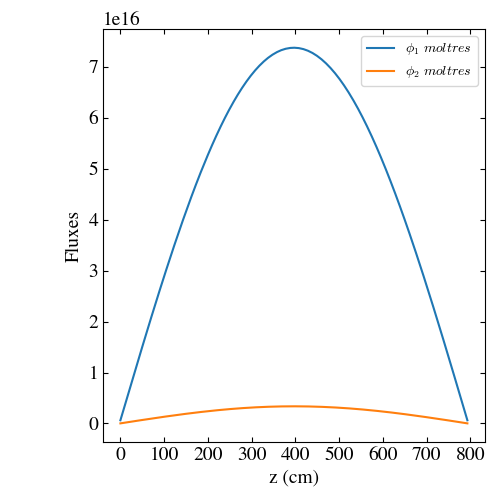
\includegraphics[height=5cm]{2D-fuel-action}
		\caption{Group 1 and 2 fluxes at 10 msec.}
		\label{fig:2D-fuel-action}
	\end{figure}

\subsection{2D-fuel-reflec-action}

	\begin{itemize}
		\item Input file: \textit{2D-fuel-reflec-action.i}
		\item Mesh: \textit{2D-fuel-reflec.msh}
		\item Transient problem.
	\end{itemize}

Figure \ref{fig:2D-fuel-reflec} shows the results.

	\begin{figure}[htbp!]
		\centering
		\begin{subfigure}[t]{0.4\textwidth}
			\centering
			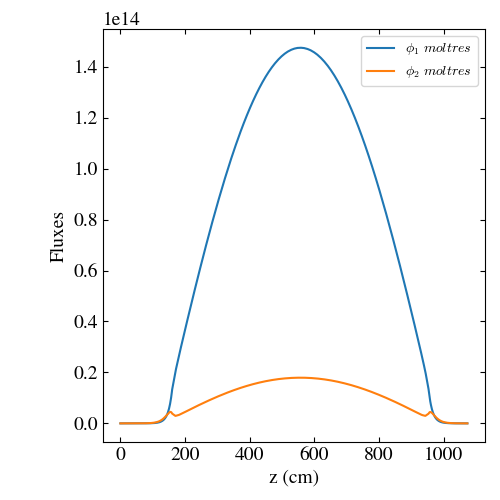
\includegraphics[width=\linewidth]{2D-fuel-reflec-action}
			\caption{Group 1 and 2 fluxes at 10 msec.}
		\end{subfigure}
		\begin{subfigure}[t]{0.4\textwidth}
			\centering
			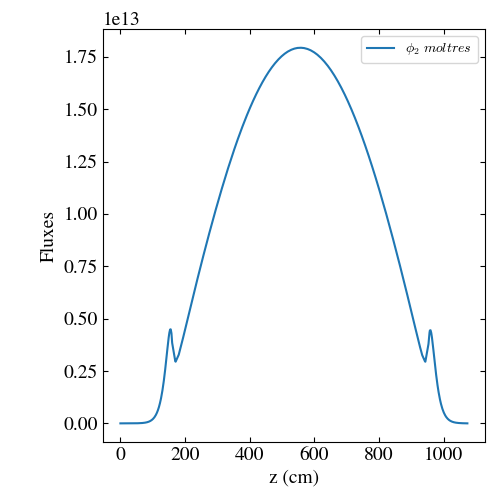
\includegraphics[width=\linewidth]{2D-fuel-reflec-action-g2}
			\caption{Group 2 flux at 10 msec.}
		\end{subfigure}
		\hfill
		\caption{Transient problem fluxes.}
		\label{fig:2D-fuel-reflec}
	\end{figure}

\subsection{2D-fuel-reflec-action-eig}

	\begin{itemize}
		\item Input file: \textit{2D-fuel-reflec-action-eig.i}
		\item Mesh: \textit{2D-fuel-reflec.msh}
		\item Eigenvalue problem: InversePowerMethod
	\end{itemize}

Figure \ref{fig:2D-fuel-reflec-action-eig} shows the results.

	\begin{figure}[htbp!]
		\centering
		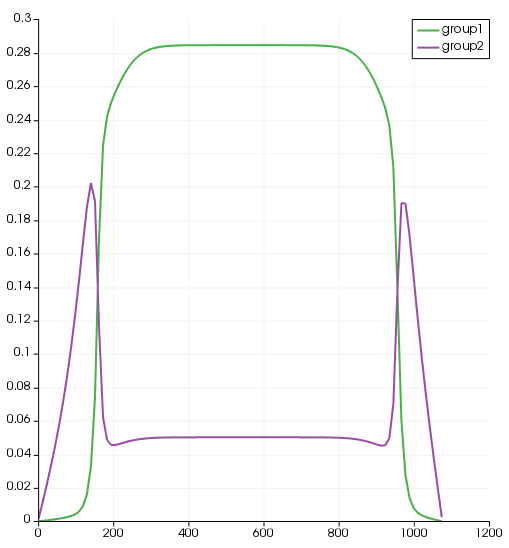
\includegraphics[height=5cm]{2D-fuel-reflec-action-eig}
		\caption{Steady state Group 1 and 2 fluxes for 'InversePowerMethod'.}
		\label{fig:2D-fuel-reflec-action-eig}
	\end{figure}

\subsection{2D-fuel-reflec-action-delayed}

	\begin{itemize}
		\item Mesh: \textit{2D-fuel-reflec.msh}
		\item Transient problem
		\item Solves for precursors
	\end{itemize}

Figure \ref{fig:2D-fuel-reflec-action-delayed} shows the results.

	\begin{figure}[htbp!]
		\centering
		\begin{subfigure}[t]{0.4\textwidth}
			\centering
			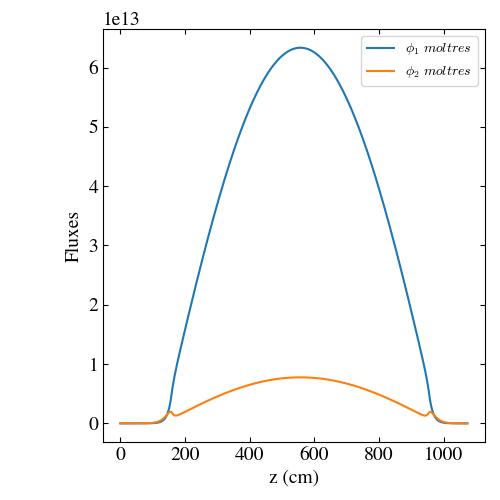
\includegraphics[width=\linewidth]{2D-fuel-reflec-action-delayed}
			\caption{Group 1 and 2 fluxes at 10 msec.}
		\end{subfigure}
		\begin{subfigure}[t]{0.4\textwidth}
			\centering
			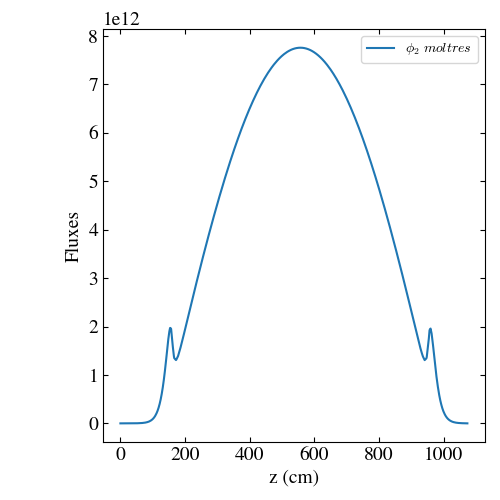
\includegraphics[width=\linewidth]{2D-fuel-reflec-action-delayed-g2}
			\caption{Group 2 flux at 10 msec.}
		\end{subfigure}
		\hfill
		\caption{Transient problem fluxes.}
		\label{fig:2D-fuel-reflec-action-delayed}
	\end{figure}

\pagebreak
\bibliographystyle{plain}
% \bibliography{bibliography}

\end{document}
